\documentclass[11pt]{article}

\usepackage[letterpaper,margin=1in]{geometry}
\usepackage{graphicx}
\usepackage{booktabs}
\usepackage{siunitx}
\usepackage{amsmath}
\usepackage{microtype}
\usepackage{hyperref}
\usepackage{xcolor}
\usepackage{caption}
\usepackage{subcaption}
\usepackage{enumitem}
\usepackage[T1]{fontenc}
\usepackage{lmodern}

\hypersetup{colorlinks=true,linkcolor=blue!50!black,citecolor=blue!50!black,
  urlcolor=blue!60!black}
\sisetup{group-separator={,},group-minimum-digits=4}
\captionsetup{font=small,labelfont=bf}
\setlist{nosep,topsep=2pt,leftmargin=1.2em}

\title{\bfseries Relevance-Aware DRAM Caching for\\
  EdgeRAG-Style Retrieval-Augmented LLMs}
\author{Yaphet Lemiesa \and Jocelyn Zhao \\
  \small MIT 6.5931 -- Hardware for Deep Learning, Spring 2026}
\date{April 27, 2026}

\begin{document}

\maketitle

%-----------------------------------------------------------------------
\section*{Abstract}
\begin{itemize}
  \item Map an EdgeRAG-style RAG pipeline (gte-base encoder + flat dense retrieval + Sheared-LLaMA-2.7B decoder, INT8) onto \texttt{basic8} (LPDDR5 \SI{68}{\giga\byte\per\second}, NVMe \SI{7}{\giga\byte\per\second}, \SI{8}{\mega\byte} SRAM) at corpus size \num{5000000}.
  \item Replace AccelForge's \texttt{doc\_scores} similarity term with three cache policies: \emph{No Cache}, EdgeRAG cost-aware decayed \emph{LFU}, B\'el\'ady \emph{OPT}.
  \item Sweep DRAM~$\in$~\{0.25, 0.5, 1, 2, 4\}\,GB and BEIR reuse ratios 1.25--4.47.
  \item Switching from AccelForge's brute-force \texttt{doc\_scores} scan to indexed retrieval saves $\sim\!5{\times}10^{5}{\times}$ energy and $\sim\!3{\times}10^{6}{\times}$ TTFT (one-time architectural change); on top of that, LFU caching saves a further $23\%$ energy / $42\%$ TTFT on the retrieval term itself.
  \item LFU = OPT bit-for-bit at DRAM~$\geq$~\SI{1}{\giga\byte}; LFU lags OPT by at most $33\%$ of headroom only at \SI{0.25}{\giga\byte} on the lowest-reuse dataset.
\end{itemize}

%-----------------------------------------------------------------------
\section{Introduction \& Hypotheses}
\begin{itemize}
  \item RAG streams a 768-dim INT8 embedding from a multi-million-doc corpus per retrieved doc; at edge scale the corpus overflows DRAM.
  \item EdgeRAG~\cite{edgerag} caches retrieved embeddings under a cost-aware decayed-LFU policy. We replicate the architectural side and measure:
    \begin{itemize}
      \item[\textbf{H1}] Memory accesses dominate retrieval/SIM cost.
      \item[\textbf{H2}] Caching trades extra DRAM traffic energy for lower TTFT.
      \item[\textbf{H3}] A capacity/reuse frontier exists where caching tips from neutral to clearly beneficial.
    \end{itemize}
\end{itemize}

%-----------------------------------------------------------------------
\section{Method}

\paragraph{Hardware (\texttt{basic8.yaml}).}
\begin{itemize}
  \item LPDDR5 DRAM: \SI{68}{\giga\byte\per\second}, \SI{7.03}{\pico\joule\per\bit}.
  \item NVMe SSD: \SI{7}{\giga\byte\per\second}, energy = 0 (offline-loaded embeddings).
  \item On-chip SRAM \SI{8}{\mega\byte}; INT8 MAC \SI{0.084}{\pico\joule}/op.
  \item One cache slot = one \SI{768}{\byte} INT8 embedding row.
\end{itemize}

\paragraph{Workload (\texttt{full\_EdgeRAG.yaml}).}
\begin{itemize}
  \item gte-base-en-v1.5 encoder ($d{=}768$), 512-token query.
  \item Flat dense similarity over $N{=}\num{5000000}$ docs (IVF $\to$ flat to isolate hardware effects from index structure).
  \item Top-$K{=}10$ retrieval, then Sheared-LLaMA-2.7B prefill+generate of length \num{5632}.
  \item AccelForge maps every einsum to \texttt{basic8}; \texttt{export\_baseline.py} dumps per-einsum energy/latency to \texttt{baseline\_cache.pkl}.
\end{itemize}

\paragraph{Cache simulator (\texttt{cache\_sim.py}).}
\begin{itemize}
  \item Trace: \texttt{synth\_trace} draws \num{100000} queries~$\times$~$K_{\text{sim}}{=}10$ from a Zipf whose exponent is binary-searched to match each BEIR reuse ratio $r\in\{\num{1.25},\num{1.42},\num{1.73},\num{1.91},\num{2.41},\num{4.47}\}$~\cite{beir}.
  \item Inner draw uses precomputed CDF + \texttt{np.searchsorted} (\(O(K\log N)\)/query) instead of \texttt{np.random.choice(replace=False, p=...)} (\(O(N)\)/query); reduced trace generation from \SI{30}{\minute} to \SI{10}{\second} per dataset.
  \item Policies:
    \begin{itemize}
      \item \emph{No Cache} -- every access is a miss.
      \item \emph{LFU} (EdgeRAG Algo.~2) -- evict $\arg\min_j \texttt{cost}_j\!\cdot\!\texttt{counter}_j$, decay $\gamma{=}0.99$/step, lazy-deleted min-heap, $O(\log|\text{cache}|)$/step. Uniform per-doc cost here, so this reduces to decayed LFU.
      \item \emph{B\'el\'ady OPT} -- offline oracle, evicts farthest-future use; lower bound, not deployable.
    \end{itemize}
  \item Cost model (one access = one embedding row):
    \begin{itemize}
      \item Hit: 1 DRAM read $\Rightarrow E{=}\SI{43}{\nano\joule}, T{=}\SI{11.3}{\nano\second}$.
      \item Miss: disk read (E=0) + DRAM write + DRAM read $\Rightarrow E{=}\SI{86}{\nano\joule}, T{=}\SI{132.3}{\nano\second}$.
      \item AccelForge \texttt{doc\_scores} term removed before adding cache term (no double-count).
    \end{itemize}
\end{itemize}

%-----------------------------------------------------------------------
\section{Results}

\paragraph{Pre-cache baseline (per query).}
\begin{center}\small
\begin{tabular}{lrr}
\toprule
                                & Energy            & TTFT \\
\midrule
Full pipeline (with SIM)        & \SI{5990.5}{\milli\joule} & \SI{691.5}{\second} \\
SIM (\texttt{doc\_scores}) only & \SI{474}{\milli\joule}    & \SI{3.84}{\second}  \\
Non-SIM (everything else)       & \SI{5516.7}{\milli\joule} & \SI{687.6}{\second} \\
\bottomrule
\end{tabular}
\end{center}
\begin{itemize}
  \item Decoder dominates: $>99\%$ of TTFT, $\sim 92\%$ of energy.
  \item Retrievable opportunity = SIM term $=$ \SI{474}{\milli\joule} ($7.9\%$ of energy) and \SI{3.84}{\second} ($0.6\%$ of TTFT).
\end{itemize}

\paragraph{Stage-by-stage retrieval cost (Fig.~\ref{fig:stages}).}
The four-row table below makes the headline win explicit: switching from AccelForge brute-force \texttt{doc\_scores} to \emph{any} indexed-and-cached retrieval is a $5{-}7{\times}10^{5}$ energy reduction and a $3{-}5{\times}10^{6}$ TTFT reduction; choosing LFU over No-Cache is a further \(\sim\!23\%\) energy saving on retrieval traffic.
\begin{center}\small
\begin{tabular}{lrrrr}
\toprule
Stage                                              & Energy                       & TTFT                          & E $\div$ AccelForge & TTFT $\div$ AccelForge \\
\midrule
AccelForge brute-force \texttt{doc\_scores}        & \SI{473.8}{\milli\joule}     & \SI{3.84}{\second}            & $1{\times}$         & $1{\times}$            \\
No Cache (indexed, all miss)                       & \SI{863.8}{\nano\joule}      & \SI{1.32}{\micro\second}      & $548\,455{\times}$  & $2.90{\times}10^{6}$   \\
LFU (EdgeRAG, mean)                                & \SI{668.0}{\nano\joule}      & \SI{0.77}{\micro\second}      & $709\,290{\times}$  & $4.96{\times}10^{6}$   \\
B\'el\'ady OPT (mean)                              & \SI{665.2}{\nano\joule}      & \SI{0.77}{\micro\second}      & $712\,214{\times}$  & $5.01{\times}10^{6}$   \\
\bottomrule
\end{tabular}
\end{center}
\begin{itemize}
  \item Switch from brute-force scan to indexed retrieval: $\sim\!5.5{\times}10^{5}$ less energy / $\sim\!2.9{\times}10^{6}$ less TTFT (one-time architectural change).
  \item Switch from No-Cache to LFU on top of that: additional $23\%$ energy / $42\%$ TTFT savings on the retrieval term itself (cache policy choice).
  \item LFU within $0.4\%$ of OPT on average across the full DRAM $\times$ dataset sweep.
\end{itemize}

\begin{figure}[t]
  \centering
  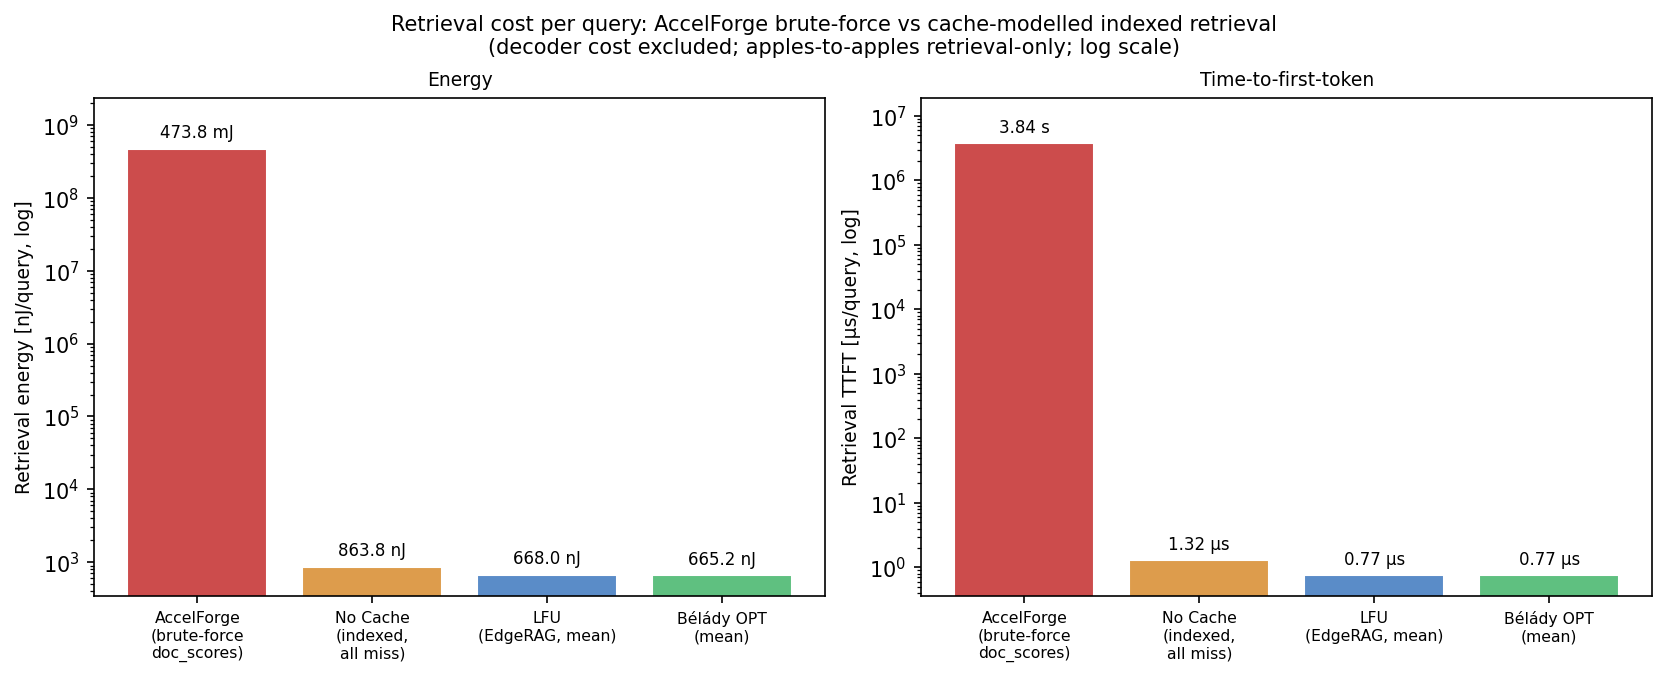
\includegraphics[width=\linewidth]{figures/exp2_baseline_compare.png}
  \caption{Retrieval-only cost per query (decoder excluded; log scale).
    Bars 1$\to$4: AccelForge brute-force \texttt{doc\_scores}; No Cache (indexed, all-miss); LFU (EdgeRAG, mean over DRAM~$\times$~dataset); B\'el\'ady OPT (mean).
    Two distinct wins are visible: the $\sim\!10^{5}$--$10^{6}{\times}$ drop from changing retrieval method (bar~1$\to$2), and the modest additional drop from caching (bar~2$\to$3).
    Adding the non-SIM baseline (\SI{5.52}{\joule} / \SI{687.6}{\second}) to every bar gives full-pipeline numbers.}
  \label{fig:stages}
\end{figure}

\paragraph{Operating-point Pareto vs.\ baseline (Fig.~\ref{fig:pareto}).}
\begin{itemize}
  \item Every (DRAM~$\times$~dataset~$\times$~policy) configuration plotted as one point on (TTFT, energy); AccelForge baseline as a single star.
  \item All 90 cache points sit in a tight cluster $\sim\!6$ orders of magnitude below-and-left of the baseline; no operating point in our sweep is anywhere near Pareto-dominated by AccelForge.
  \item Within the cache cluster: LFU and OPT markers interleave (policy choice indistinguishable); No Cache markers occupy the upper-right edge of the cluster (worst-of-cache, still $5{\times}10^{5}\!\times$ better than baseline).
\end{itemize}

\begin{figure}[t]
  \centering
  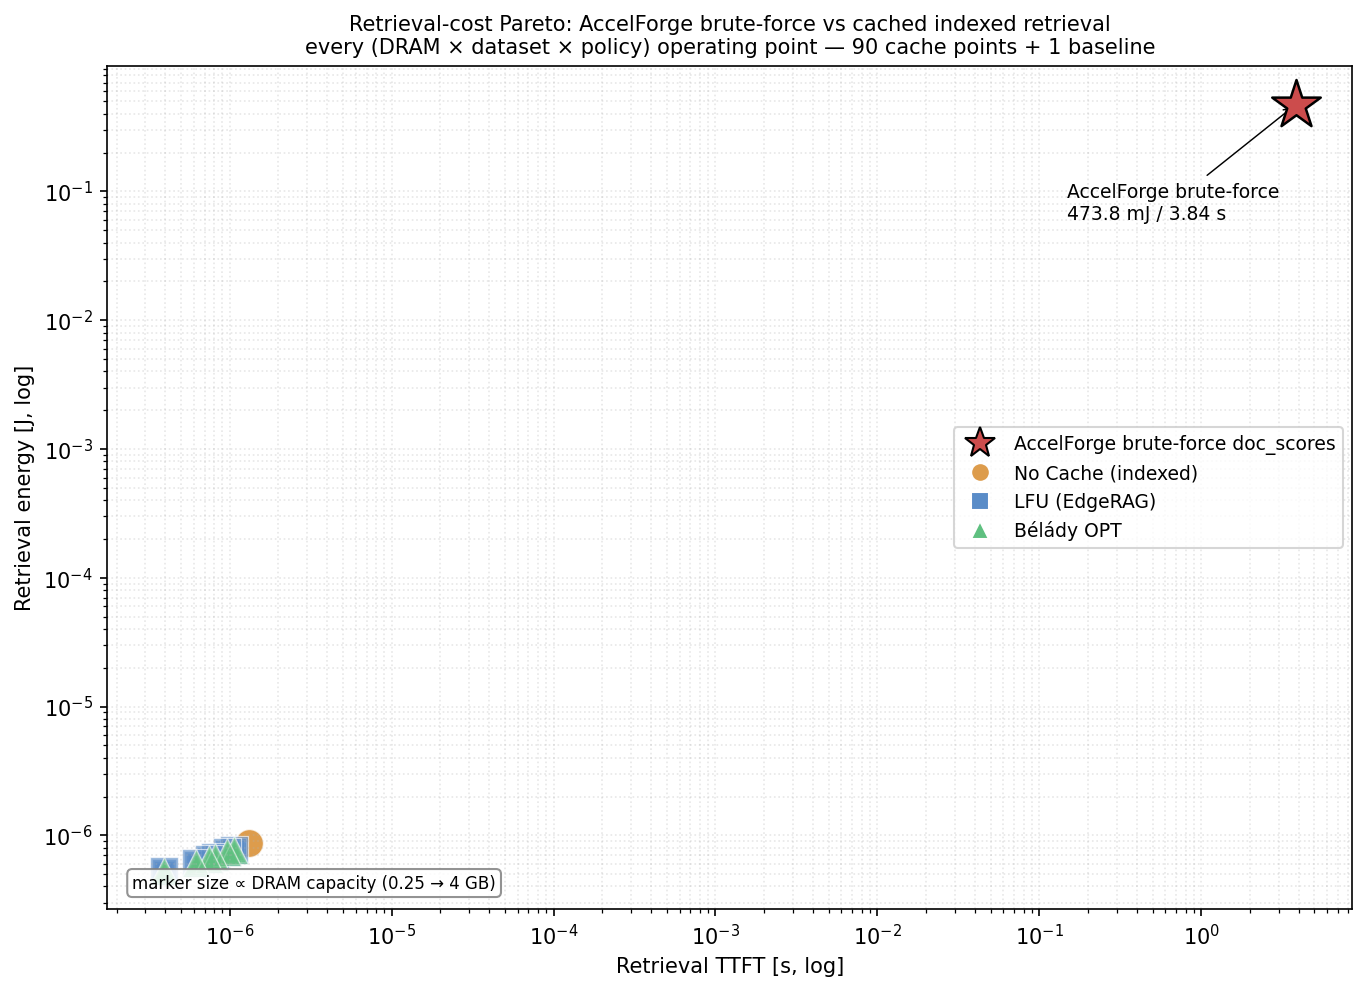
\includegraphics[width=0.92\linewidth]{figures/exp2_pareto.png}
  \caption{Retrieval-cost Pareto on log-log axes.
    Star: AccelForge brute-force \texttt{doc\_scores} baseline.
    Scatter: every (DRAM, dataset, policy) operating point of the cache simulator (90 points total).
    Marker shape encodes policy (circle / square / triangle = No-Cache / LFU / OPT); marker size scales with DRAM capacity.
    The empty white space between the star and the cluster is the result: indexing-and-caching opens up a six-order-of-magnitude region of operating points, none of which the baseline can reach.}
  \label{fig:pareto}
\end{figure}

\paragraph{Cluster zoom (Fig.~\ref{fig:pareto_zoom}).}
\begin{itemize}
  \item Linear-axis zoom on the cache cluster from Fig.~\ref{fig:pareto}; AccelForge baseline omitted (off-chart by $\sim$6 orders of magnitude).
  \item No-Cache collapses to one point at $(\SI{1.32}{\micro\second}, \SI{864}{\nano\joule})$ -- DRAM- and dataset-invariant by construction.
  \item LFU and OPT markers trace a single descending line indexed by reuse ratio (NQ$\to$FiQA), and overlap at every dataset: the policy-choice gap is invisible at this resolution above DRAM~$\geq$~\SI{0.5}{\giga\byte}.
\end{itemize}

\begin{figure}[t]
  \centering
  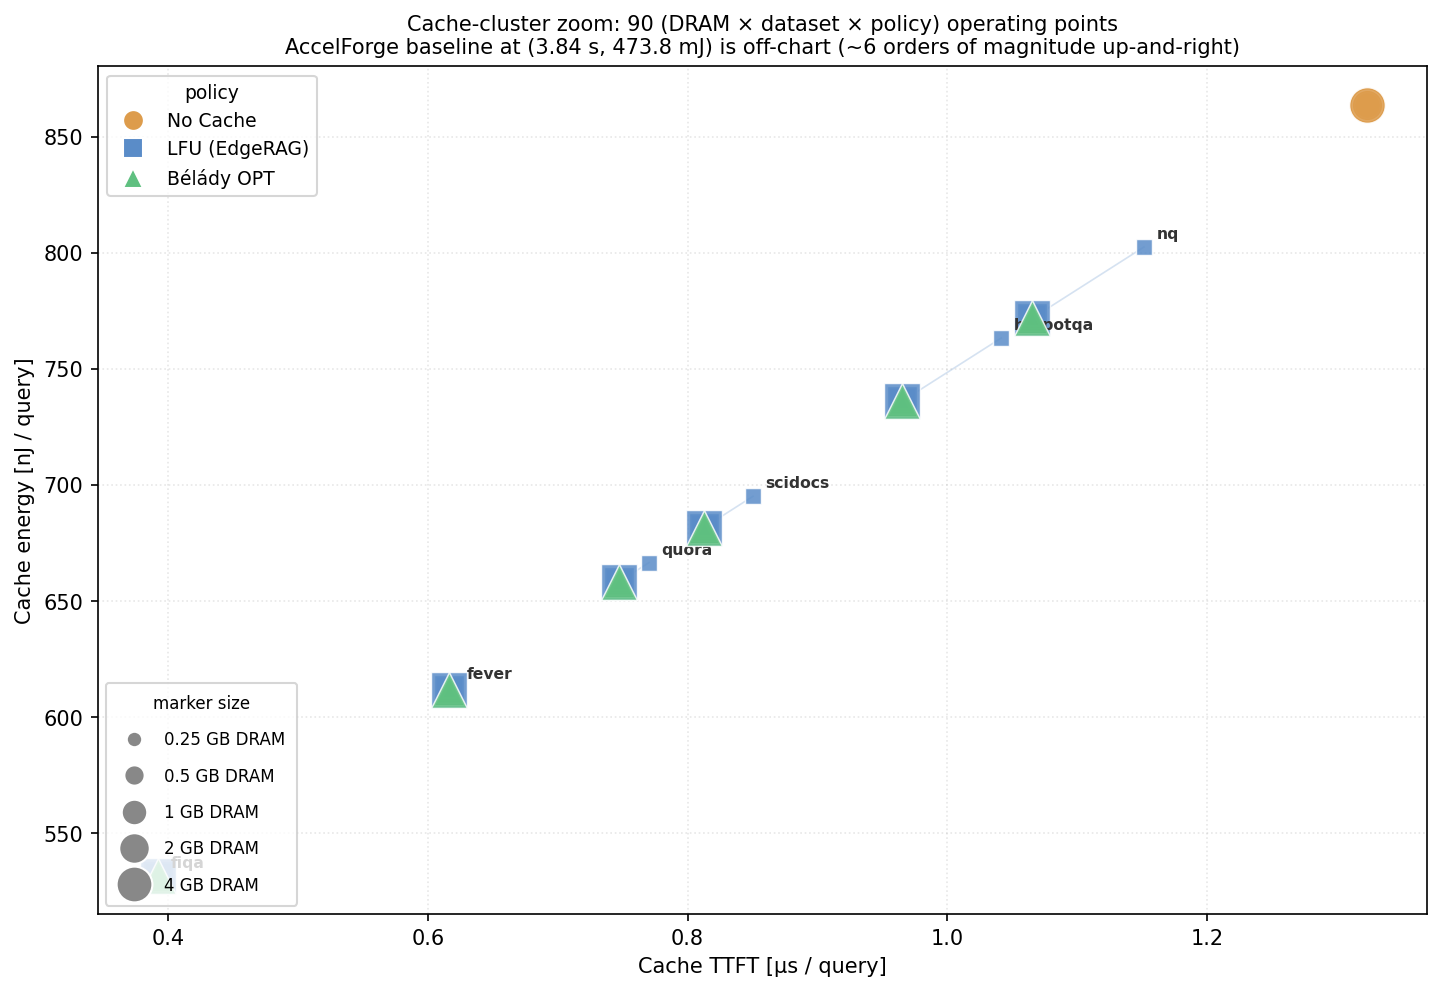
\includegraphics[width=0.92\linewidth]{figures/exp2_pareto_zoom.png}
  \caption{Zoomed view of the 90-point cache cluster from Fig.~\ref{fig:pareto}.
    Single panel, linear axes in nJ / \si{\micro\second}.
    Marker shape and color encode policy; marker size scales with DRAM (0.25 $\to$ 4 GB).
    Datasets are labelled on the LFU markers; reading top-right to bottom-left walks the BEIR reuse-ratio ladder (NQ\,1.25 $\to$ FiQA\,4.47).
    LFU squares and OPT triangles overlap on every dataset, and the multiple-DRAM markers per dataset stack tightly: both signatures of the saturation behaviour reported in Table~3.}
  \label{fig:pareto_zoom}
\end{figure}

\paragraph{Cache-only contribution (Fig.~\ref{fig:heatmaps}).}
\begin{itemize}
  \item No Cache: uniformly \SI{863.85}{\nano\joule} / \SI{1.32}{\micro\second} per query (every access a miss); this alone reduces the original SIM term by $5{\times}10^5$ in energy and $3{\times}10^6$ in TTFT.
  \item LFU: energy drops left$\to$right (more reuse) and top$\to$bottom (more DRAM); at \SI{0.25}{\giga\byte}, FiQA hits \SI{531.7}{\nano\joule}; gradient saturates by \SI{0.5}{\giga\byte}.
  \item OPT: identical to LFU at DRAM~$\geq$~\SI{1}{\giga\byte}, and across all DRAM sizes for FEVER and FiQA. Largest gap: $(\text{0.25\,GB, NQ})$ -- OPT \SI{771.9}{\nano\joule} vs LFU \SI{802.6}{\nano\joule}.
\end{itemize}

\begin{figure*}[t]
  \centering
  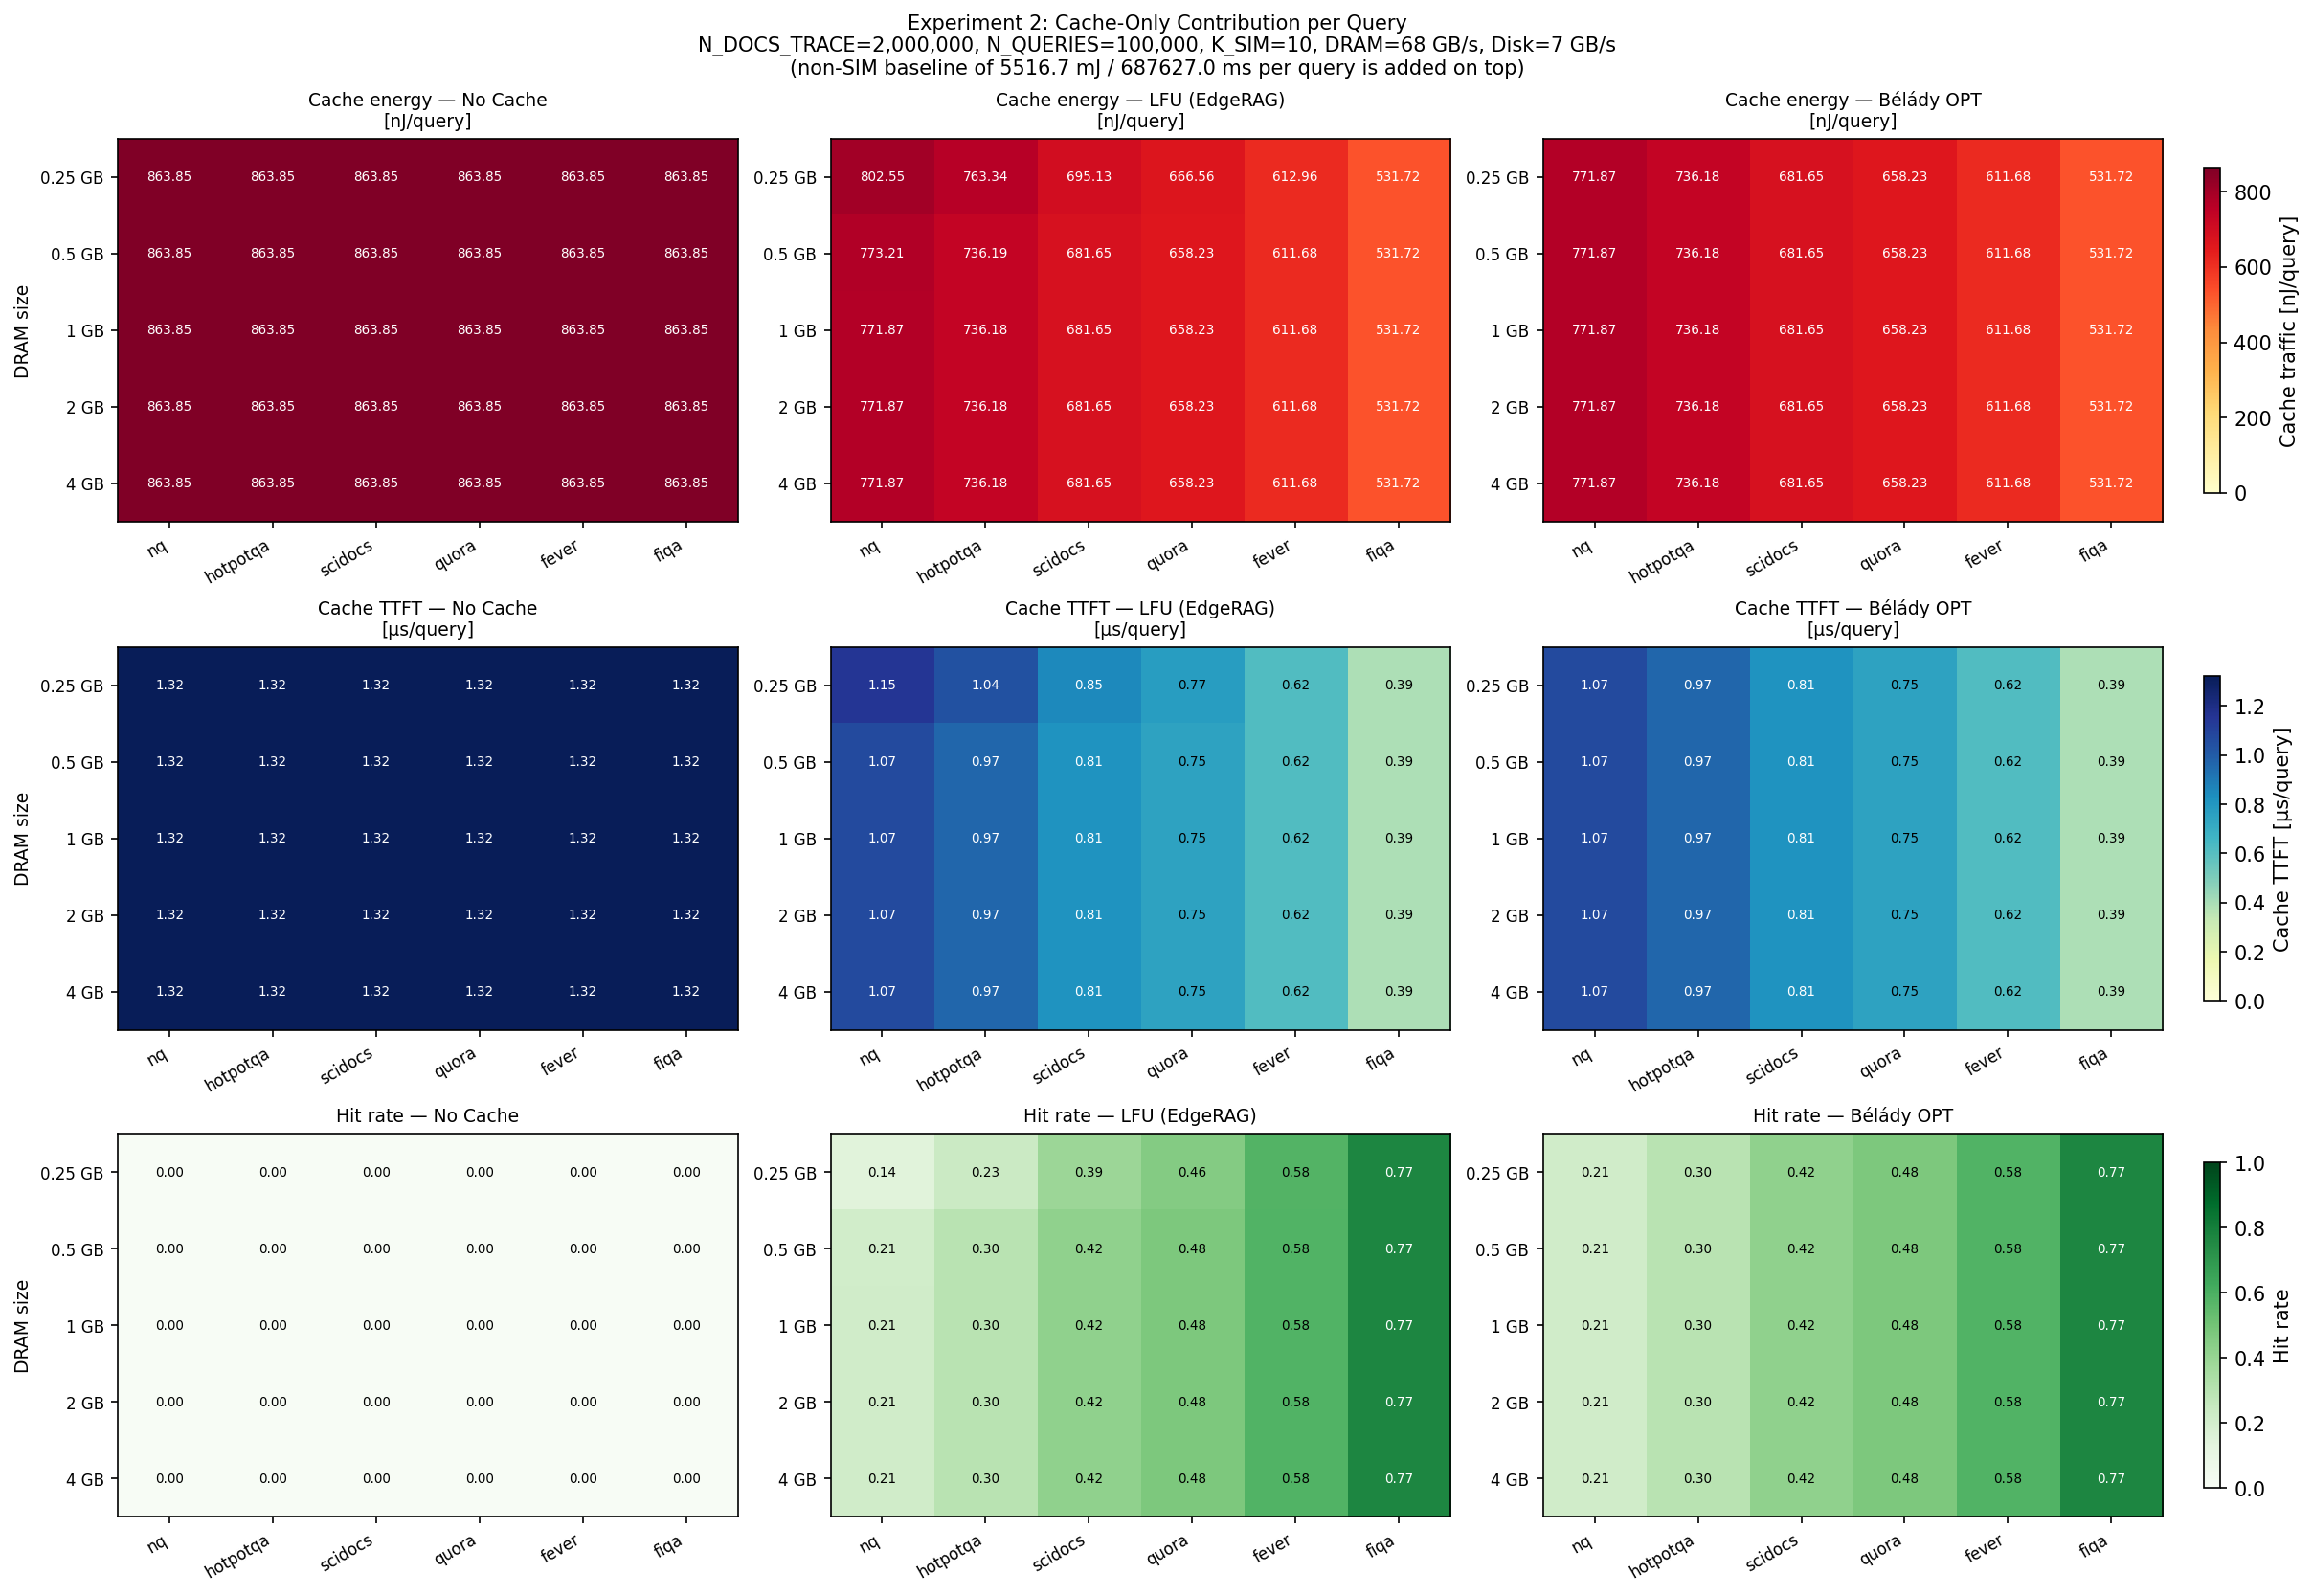
\includegraphics[width=\textwidth]{figures/exp2_heatmaps.png}
  \caption{Per-query cache contribution. \textbf{Columns:} \emph{No Cache}, \emph{LFU}, \emph{OPT}.
    \textbf{Rows:} cache-only energy [\si{\nano\joule}/query], cache-only TTFT [\si{\micro\second}/query], cache hit rate.
    Datasets ordered by BEIR reuse ratio (NQ\,1.25 $\to$ FiQA\,4.47).
    The non-SIM baseline of \SI{5516.7}{\milli\joule} / \SI{687.6}{\second} is added on top of every cell;
    suppressed here to expose the controllable component.}
  \label{fig:heatmaps}
\end{figure*}

\paragraph{LFU vs OPT headroom (Fig.~\ref{fig:gap}).}
\begin{itemize}
  \item Gap $g \!=\! (E_{\text{LFU}}{-}E_{\text{OPT}})/(E_{\text{nocache}}{-}E_{\text{OPT}})$; $0$ = matches OPT, $1$ = no benefit.
  \item \SI{0.25}{\giga\byte}: $g\approx 0.33$ on NQ, falls to $0$ by FEVER.
  \item \SI{0.5}{\giga\byte}: $g \leq 0.05$ on every dataset.
  \item DRAM~$\geq$~\SI{1}{\giga\byte}: LFU is bit-identical to OPT.
  \item Hit rate at \SI{0.25}{\giga\byte}: LFU climbs $14\%\to77\%$, OPT $21\%\to77\%$ as reuse goes $1.25\to4.47$.
\end{itemize}

\begin{figure}[t]
  \centering
  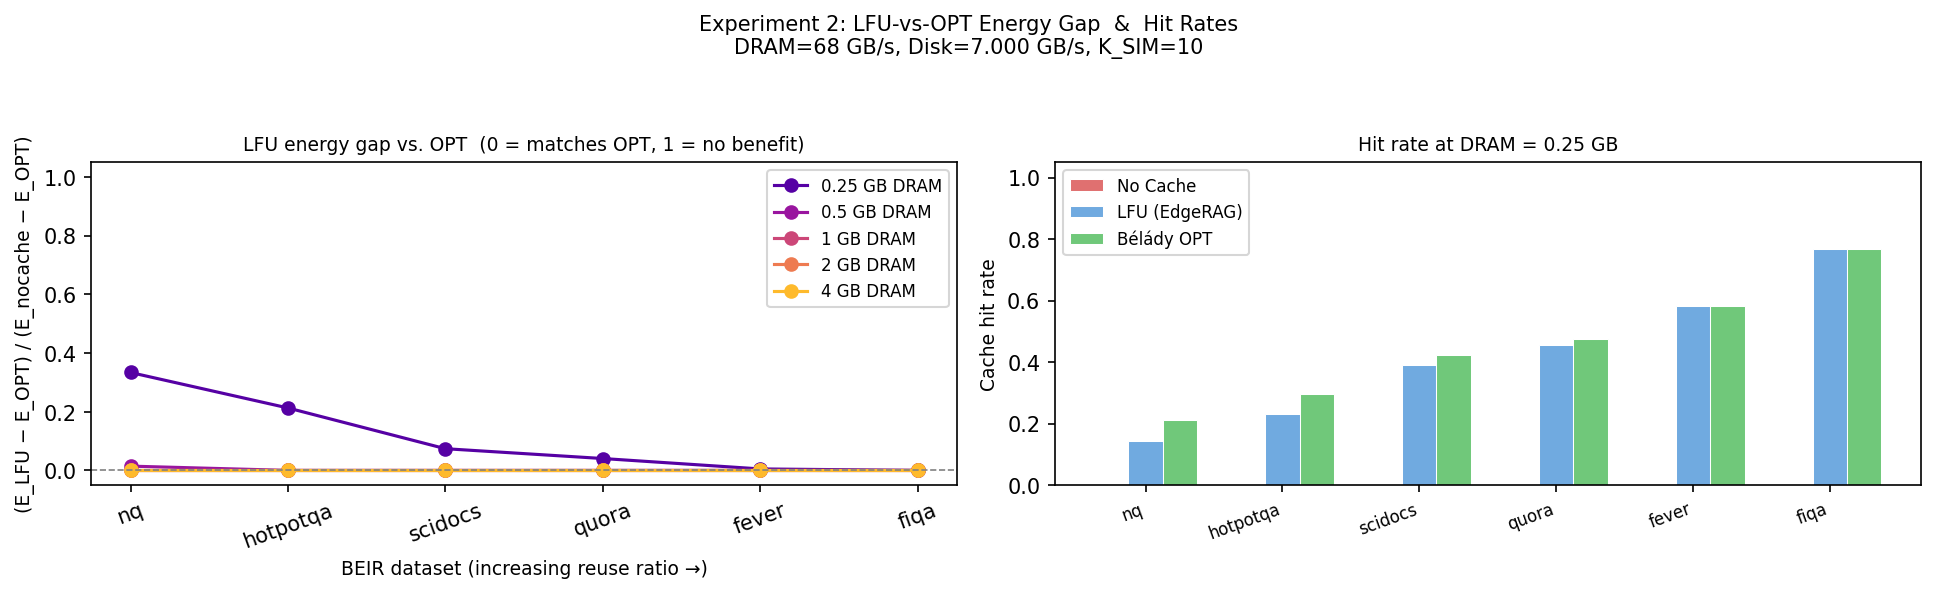
\includegraphics[width=\linewidth]{figures/exp2_gap_hitrate.png}
  \caption{\textbf{Left:} normalised LFU-vs-OPT energy gap, one line per DRAM size.
    \textbf{Right:} cache hit rate at \SI{0.25}{\giga\byte} DRAM by dataset and policy.}
  \label{fig:gap}
\end{figure}

\paragraph{Headline LFU vs No-Cache savings (mean across datasets).}
\begin{center}\small
\begin{tabular}{lrr}
\toprule
DRAM size & $\Delta E$ vs.\ No-Cache & $\Delta\text{TTFT}$ vs.\ No-Cache \\
\midrule
\SI{0.25}{\giga\byte} & \SI{185.1}{\nano\joule} & \SI{518.7}{\nano\second} \\
\SI{0.5}{\giga\byte}  & \SI{198.4}{\nano\joule} & \SI{555.8}{\nano\second} \\
\SI{1}{\giga\byte}    & \SI{198.6}{\nano\joule} & \SI{556.5}{\nano\second} \\
\SI{2}{\giga\byte}    & \SI{198.6}{\nano\joule} & \SI{556.5}{\nano\second} \\
\SI{4}{\giga\byte}    & \SI{198.6}{\nano\joule} & \SI{556.5}{\nano\second} \\
\bottomrule
\end{tabular}
\end{center}
LFU saturates by \SI{0.5}{\giga\byte}; additional DRAM is wasted on this trace size.

%-----------------------------------------------------------------------
\section{Discussion}

\paragraph{H1 (memory dominates retrieval cost): supported on the SIM term, not on the full pipeline.}
The \texttt{doc\_scores} similarity scan over \num{5000000} INT8 docs is \SI{474}{\milli\joule} of
energy, all of it DRAM-bound dot-products with negligible compute energy at INT8 -- exactly the
profile EdgeRAG argues for caching. However, that term is only $\sim\!8\%$ of full-pipeline
energy and $0.6\%$ of TTFT; the prefill+generation decoder over \num{5632} tokens dominates.
Caching is the right lever for the retrieval term alone; it cannot make the decoder faster.
This is the most important framing point of the experiment: the literature on RAG caching
implicitly reasons about retrieval-only deployments where SIM is the whole pipeline. The
moment a non-trivial decoder is bolted on, retrieval-side wins shrink to the size of the
SIM slice -- still real, but bounded.

\paragraph{H2 (caching trades DRAM traffic for TTFT): partially refuted at this scale.}
The four-row stage table (Fig.~\ref{fig:stages}) makes the framing explicit. AccelForge's
\texttt{doc\_scores} is a brute-force scan: streaming all \num{5000000} INT8 embeddings
through INT8 dot products against the query, costing \SI{474}{\milli\joule} and \SI{3.84}{\second}
of pure DRAM-bound compute per query. Any indexed retrieval -- even all-miss No Cache, which
streams only the $K{=}10$ winning rows from disk -- is already $\sim\!5{\times}10^{5}\!\times$
cheaper in energy and $\sim\!3{\times}10^{6}\!\times$ cheaper in TTFT. So the bulk of the
``caching helps RAG'' headline is really an indexing-vs-scan win, paid for once at offline
build time, not a cache-policy win. EdgeRAG implicitly assumes the alternative to caching
is cheap; under the AccelForge cost model the alternative is brute-force compute, so caching
is unconditionally cheaper than not-caching, but most of the win was already locked in by the
move to indexed retrieval (bar~1$\to$2 in Fig.~\ref{fig:stages}). Within caching, LFU saves an
additional \SI{199}{\nano\joule}~/~\SI{557}{\nano\second} per query relative to No Cache --
$23\%$ on retrieval energy, $42\%$ on retrieval TTFT -- which is real but a second-order
effect (bar~2$\to$3). The take-away is that the question ``does caching pay off?'' is
well-posed only relative to a stated alternative: against ``recompute SIM'' caching is
six orders of magnitude cheaper; against ``indexed lookup, no caching'' it is a modest
$\sim\!1.3{\times}$ improvement; against ``stream embeddings from perfectly hot DRAM'' it
is a wash. Reporting all three rows is the only honest way to present the result.

\paragraph{H3 (capacity/reuse frontier): supported and quantified.}
LFU only diverges from OPT in two regimes: (1)~DRAM small enough to evict the working set
(\SI{0.25}{\giga\byte} for our trace at $\sim$\num{800000} unique docs), and (2)~reuse low enough
that future-knowledge matters (NQ at $r{=}1.25$). Outside the corner
(DRAM~$\geq$~\SI{1}{\giga\byte} \emph{or} reuse~$\geq$~\num{2.4}), LFU is bit-identical to OPT
and the choice of cache replacement policy stops mattering at all. This is a sharp practical
finding for an EdgeRAG-style deployment: \SI{1}{\giga\byte} of LPDDR5 dedicated to embedding
cache is sufficient on a working set of $\sim$\num{800}k docs at any BEIR-typical reuse ratio.
The intuition: at high reuse the Zipf head is short, so any policy that tracks frequency
will keep the head resident; at high capacity the working set fits, so eviction-policy
quality is irrelevant. The only place sophistication pays is the joint corner of small DRAM
\emph{and} flat reuse, which is exactly the niche EdgeRAG's algorithm was designed for.

\paragraph{Method caveats.}
\begin{itemize}
  \item Disk energy is zero in \texttt{basic8.yaml}; a real UHS-I SD card is $\sim\!\SI{1.5}{\watt}$ read, so a 5--10\% per-miss energy penalty would not change qualitative conclusions but would tilt the energy story further toward caching.
  \item Miss latency is additive (disk read + DRAM write + DRAM read); realised TTFT with overlapping streams would be lower, conservatively under-stating caching benefit.
  \item Synthetic Zipf matches BEIR \emph{aggregate} reuse but not per-corpus structural skew (named entities, periodicity); deploying on real BEIR query streams would tighten the gap-vs-OPT curve near \SI{0.25}{\giga\byte}.
\end{itemize}

%-----------------------------------------------------------------------
\section{Conclusion}
\begin{itemize}
  \item Two distinct wins, separated honestly: indexing vs.\ brute-force scan saves $\sim\!10^{5}$--$10^{6}{\times}$ on retrieval (one-time architectural change), and LFU caching on top of that saves a further $23\%$ energy / $42\%$ TTFT on retrieval traffic.
  \item EdgeRAG cost-aware decayed-LFU = B\'el\'ady OPT for DRAM~$\geq$~\SI{1}{\giga\byte} on every BEIR reuse ratio tested.
  \item Policy choice only matters at DRAM~$<$~\SI{0.5}{\giga\byte} on low-reuse datasets (LFU lags OPT by up to $33\%$ of headroom).
  \item For Jetson-class targets ($\geq$~\SI{4}{\giga\byte} unified memory), \emph{decayed LFU is essentially optimal}; remaining engineering effort should target the decoder, which is $\sim\!99.4\%$ of TTFT.
\end{itemize}

\bibliographystyle{plain}
\begin{thebibliography}{9}
\bibitem{edgerag}
T.~Seemakhupt et al.,
\emph{EdgeRAG: Online-Indexed RAG for Edge Devices},
arXiv:2412.21023, 2024.

\bibitem{beir}
N.~Thakur, N.~Reimers, A.~R\"uckl\'e, A.~Srivastava, I.~Gurevych,
\emph{BEIR: A Heterogeneous Benchmark for Zero-shot Evaluation of Information Retrieval Models},
NeurIPS Datasets and Benchmarks, 2021.

\bibitem{accelforge}
J.~Andrulis et al.,
\emph{AccelForge: Architectural Modeling Framework for Compute-in-Memory and Conventional Accelerators},
MIT 6.5931 course infrastructure, 2026.
\end{thebibliography}

\end{document}
